\xchapter{Introdução}{}

\acresetall 


Este capítulo apresenta o contexto em que a presente investigação se insere, enfatizando: a apresentação; o problema; os objetivos; as questões de pesquisa; a metodologia; os resultados esperados e como o trabalho está estruturado.

\section{Apresentação}\label{sec:apresentacao}
Desenvolver software não é uma tarefa simples e envolve diversas condicionais, tais como: escopo, prazo e recursos disponíveis. Nesse processo, um problema que pode ocorrer é entregar algo diferente do que era esperado pelo cliente. Isso acontece na maioria das vezes porque as atividades de desenvolvimento dependem da capacidade de interpretação e execução das pessoas que as constroem. Para que esses erros não perdurem e para que se possa identificá-los antes de liberar o software para utilização, existe uma série de atividades, coletivamente chamadas de Validação, Verificação e Teste \cite{DELAMARO2007}. 

\ac{VV} permite que se determine sistematicamente se os requisitos de um sistema estão sendo corretamente tratados e implementados. A atividade de testes tem por objetivo descobrir defeitos no software, considerando aspectos estruturais e lógicos. Verificar, validar e testar software auxiliam na Garantia de Qualidade do mesmo. Garantia de Qualidade, do termo comumente utilizado (em inglês) \ac{QA}, é o processo geral de definição de como a qualidade de software pode ser alcançada, e como a organização de desenvolvimento sabe que o software tem o nível de qualidade necessário. \ac{QA} estabelece processos, procedimentos e padrões que conduzem a um software de qualidade \cite{HIRAMA2011}. 

O presente trabalho tem como foco a atividade de teste. Os testes são normalmente executados e reportados durante as etapas de desenvolvimento do software. Espera-se que haja uma grande massa de testes realizada antes de se disponibilizar uma versão estável do software. Entretanto, existe uma técnica de testes, denominada \textbf{teste de regressão}, que deve ser considerada quando é necessário realizar a manutenção do software, quer perfectiva, corretiva, adaptativa ou preventiva \cite{DBLP:series/springer/Mens08}. O teste de regressão tem como objetivo fornecer confiança de que as alterações recém-introduzidas não obstruem os comportamentos da parte existente e inalterada do software \cite{Yoo:2012:RTM:2284811.2284813}.

No teste de regressão, há a reexecução de todos os casos de testes da versão original do software. Esse procedimento tende a gerar um grande esforço da equipe de testes, a depender da quantidade de casos de teste. A literatura apresenta uma série de técnicas para lidar com este problema, em particular no sentido de propor mecanismos para reduzir o número de reexecuções de casos de testes, sem perder a cobertura do código fonte e a capacidade de detecção de falhas ,\cite{65194}, \cite{WHITE1991}, \cite{Graves:2001:ESR:367008.367020}, \cite{630875}, \cite{536955}, \cite{ENGSTROM201014},\cite{ENGSTROM201014}, \cite{KAZMI2017}, \cite{ROMANO201862}. Segundo \citeonline{Yoo:2012:RTM:2284811.2284813} as técnicas de Teste de Regressão são classificadas como: Técnicas de Seleção; Técnicas de Minimização; e Técnicas de Priorização.  

Dentre os domínios de aplicação emergentes, testes de regressão apresentam-se como uma estratégia viável para lidar com a complexidade - e a constante evolução - dos \ac{APPS}. Neste cenário, o presente trabalho tem como foco a análise da evolução das técnicas de seleção de teste de regressão no desenvolvimento de \ac{APPS} para Android.


\section{Problema}\label{sec:problema}

Os dispositivos móveis tem sido cada vez mais utilizados no cotidiano, em alguns casos com maior parcela de mercado do que os tradicionais Desktop \cite{Do2016RedroidAR}. Pesquisas de mercado recentes indicam que o \textbf{Android} é o sistema operacional mais popular para os dispositivos móveis - vide Figura \ref{fig:marketShare}\footnote{\url{http://gs.statcounter.com/os-market-share/mobile/worldwide}}. 

Segundo \citeonline{Do2016RedroidAR}, a plataforma móvel está se separando de uma variedade de áreas de aplicativos de Desktop, tais como entretenimento, comércio eletrônico e mídia social. Assim, os desenvolvedores são obrigados a produzir \ac{APPS} de alta qualidade, em particular no que diz respeito a requisitos não-funcionais como portabilidade, confiabilidade e segurança.


\begin{figure}
    \centering
    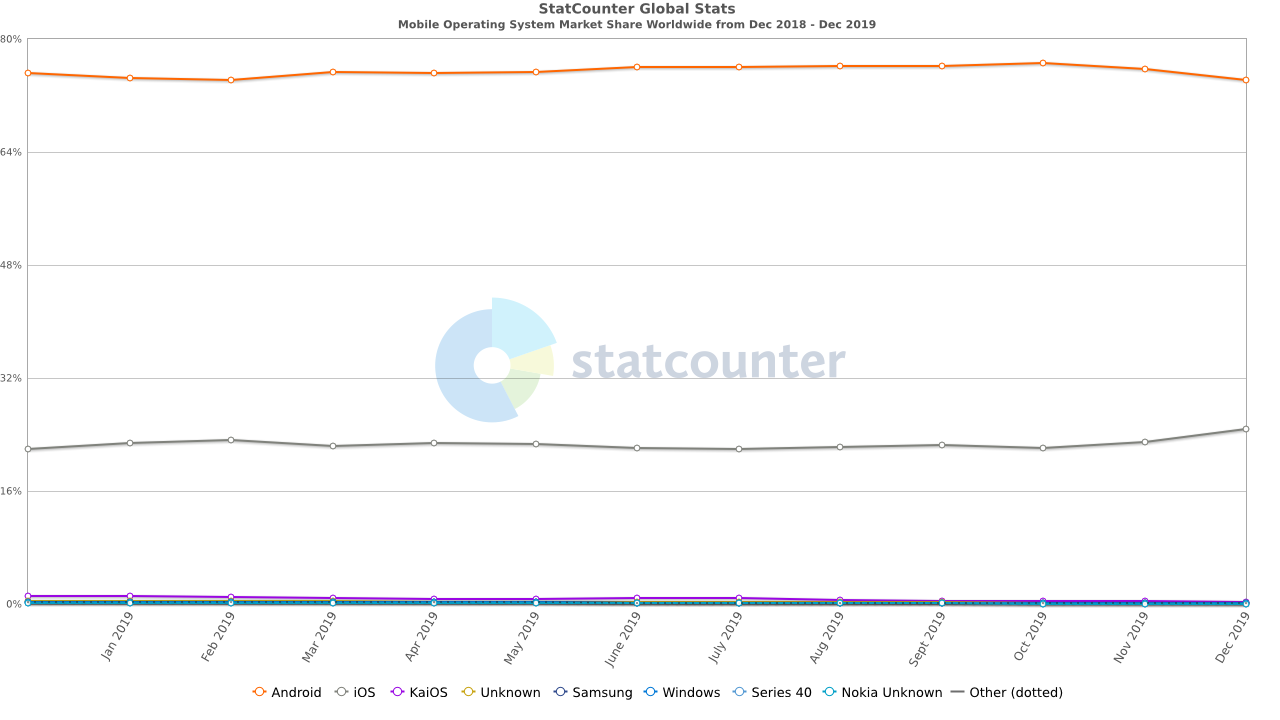
\includegraphics[width=1.\textwidth]{images/StatCounter-os_2020.png}
    \caption{Distribuição mundial do uso de sistemas operacionais para \ac{APPS}.}
    \label{fig:marketShare}
\end{figure}


Nos últimos anos, uma grande quantidade de pesquisas tem sido realizada para prover uma maior confiabilidade dos \ac{APPS}, por exemplo, aplicando testes automatizados \cite{7927972}, \cite{8424973},\cite{8453877}. No entanto, a maioria das pesquisas está focada no teste de uma versão única de aplicativos móveis \cite{Do2016RedroidAR}. Como os \ac{APPS} evoluem com frequência, é importante que os desenvolvedores façam uso de técnicas de teste de regressão, dado seu potencial em identificar problemas no código decorrentes de mudanças no software \cite{8377661}.


Ao tratar de técnicas de teste de regressão, a literatura apresenta diversos trabalhos que fazem uso de técnicas tradicionais, i.e., concebidas para testar sistemas Desktop \cite{536955}, \cite{ENGSTROM201014}. Entretanto, embora muitas abordagens eficientes e eficazes tem sido propostas, há pouca evidência indicando a aplicação direta dessas técnicas para o teste de \ac{APPS} \cite{Do2016RedroidAR}. Um importante fator que causa a incompatibilidade é a diferença entre a arquitetura do sistema da plataforma móvel e a plataforma Desktop.

Segundo \citeonline{5954416}, a qualidade dos \ac{APPS} é geralmente ruim. Um dos fatores da falta de qualidade são processos de desenvolvimento muito rápidos em que a atividade de teste é negligenciada ou conduzida de forma superficial, uma vez que é considerada demasiado complexa, difícil de automatizar, dispendiosa e demorada. 

Em virtude do crescimento do mercado de dispositivos móveis e da necessidade de produzir \ac{APPS} com qualidade, pesquisas recentes tem apresentado o desenvolvimento de técnicas implementadas por ferramentas de teste de regressão voltadas para aplicações em Android \cite{Do2016RedroidAR}, \cite{Choi:2018:DMA:3180155.3180173}, \cite{8377661}, \cite{5954416}, \cite{7927972}, \cite{8424973}, \cite{6339502}, \cite{6569773}, \cite{7427895}, \cite{7832883}, \cite{7833000}. Alguns desses estudos tratam de experimentos com comprovação empírica para comprovar a eficiência/eficácia da ferramenta proposta neste cenário.

Embora a literatura tenha dedicado esforços à produzir evidências sobre a criação de novas técnicas de teste de regressão para Android, os estudos existentes são bastante limitados no que diz respeito a demonstrar evidências empíricas que garantam quais são as técnicas de seleção de teste de regressão implementadas por ferramentas mais aplicáveis no desenvolvimento de \ac{APPS} Android. Neste sentido, é fundamental que novas pesquisas sejam desenvolvidas, de modo a ampliar o conjunto de evidências sobre essa aplicabilidade. 

Dado a complexidade do problema ora descrito, este estudo buscará responder à seguinte questão de pesquisa principal:
\leavevspace 

\begin{center}
    \noindent\fbox{ 
        \parbox{.8\textwidth}
        {
        \begin{center}
            
            \textbf{Quais são as técnicas de seleção de teste de regressão implementadas por ferramentas adequadas para projetos de \ac{APPS} Android?}
        \end{center}
        }
    }
\end{center}

\vspace{.5em}

Esta questão foi refinada em questões específicas:
\vspace{.5em}

\begin{enumerate}[label=\bf QP\arabic*,leftmargin=1.8cm]
    
    \item \textbf{Quais são as técnicas de seleção de teste de regressão apresentadas na literatura?} Essa questão de pesquisa será respondida com a revisão estruturada da literatura sobre Técnicas de Seleção de Teste de Regressão.
    
    \item \textbf{Existem ferramentas de teste de regressão aplicadas a \ac{APPS} Android disponíveis para utilização (open source ou proprietárias) implementadas a partir de técnicas de seleção de teste de regressão?} Essa questão de pesquisa será respondida com a revisão estruturada da literatura sobre ferramentas de teste de regressão.
    
    \item \textbf{Qual a perspectiva de acadêmicos e profissionais sobre técnicas de seleção de teste de regressão implementadas por ferramentas para projetos de \ac{APPS} Android?} Essa questão de pesquisa será respondida com a aplicação de um \textit{Survey} e de realização de Entrevistas com estudantes/profissionais que atuam em projetos de apps Android.

\end{enumerate}



\subsection{Objetivos}

Compreendendo que o estudo das técnicas de seleção de teste de regressão para Android é um campo em expansão, o presente trabalho tem como objetivo \textbf{realizar uma avaliação empírica das técnicas de seleção de teste de regressão implementadas por ferramentas aplicadas a \ac{APPS} Android.}

Os seguintes objetivos específicos foram definidos para esta investigação:

\begin{enumerate}[label=\bf O\arabic*,leftmargin=1.5cm]

    \item \textbf{Levantar quais são as técnicas de seleção de teste de regressão que a literatura apresenta.} Para alcançar esse objetivo, será realizado uma revisão estruturada de literatura sobre técnicas de seleção de teste de regressão.
    
    \item \textbf{Verificar quais são as ferramentas de teste de regressão aplicadas a \ac{APPS} Android disponíveis para uso (open source ou proprietárias), e se as mesmas foram implementadas baseadas nas técnicas de seleção de teste de regressão.} Para alcançar esse objetivo, será realizado uma revisão estruturada de literatura sobre ferramentas de teste de regressão.
    
    \item \textbf{Identificar como é realizado o processo de teste de software por acadêmicos e profissionais que desenvolvem \ac{APPS} Android.} Para alcançar esse objetivo, será aplicado um \textit{Survey} e realizado entrevistas com acadêmicos e profissionais que trabalham com projetos de \ac{APPS} para Android.


\end{enumerate}



\section{Metodologia}\label{sec:metodologia}


Esta Seção apresenta a metodologia utilizada para desenvolver este trabalho e alcançar os objetivos propostos:


\begin{itemize}
  \item \textbf{Fase 1}: Etapa conceitual que tem como objetivo tratar dos conhecimentos referentes ao tema proposto.
  
  
  Esta etapa visa levantar a bibliografia das áreas sob investigação, para compreender conceitos fundamentais. São elas: evolução de software; qualidade de software; testes de software; teste de regressão; técnicas de seleção; estratégias de testes de aplicações para dispositivos móveis; ferramentas para teste de \ac{APPS} Android.
  
  O levantamento bibliográfico foi feito de forma estruturada, com a leitura de livros e artigos sobre os tópicos abordados na pesquisa. Inicialmente uma leitura mais ampla em busca de um conhecimento inicial, e em uma segunda fase, com leituras específicas de textos com relação direta a este trabalho.
  
  \item \textbf{Fase 2}: Refere-se ao Survey.
  
  Esta etapa contempla a aplicação de um Survey para acadêmicos e profissionais que trabalham com \ac{APPS} Android, para compreender como é realizado o processo de teste de \ac{APPS} Android.
  
  \item \textbf{Fase 3:} Refere-se as Entrevistas.
  
  Esta etapa refere-se a realização de entrevistas com uma amostra de profissionais que trabalham no processo de testes de \ac{APPS} Android e possuem experiência na área, para compreender questões específicas referente a este processo.
  
  \item \textbf{Fase 4}: Refere-se ao Estudo Experimental.
  
  Esta etapa contempla a execução de um estudo experimental cujo objetivo principal é compreender quais são as técnicas de teste de regressão implementadas por ferramentas disponíveis mais adequadas para projetos de \ac{APPS} Android. 
  
\end{itemize}

\section{Resultados Esperados}\label{sec:resultadosesperados}

Ao final deste trabalho, espera-se contribuir com os seguintes resultados:


\begin{itemize}

    \item Contribuir com o corpo de conhecimento sobre o uso de técnicas de seleção para o desenvolvimento de \ac{APPS} Android, com base na síntese de evidências disponíveis na literatura.
    
    \item Coletar e analisar dados, no sentido de prover evidências empíricas sobre quais as técnicas de seleção implementadas por ferramentas são mais adequadas para projetos de \ac{APPS} Android.
    
    \item Identificar a perspectiva de profissionais / estudantes no que refere-se a aplicação das técnicas de seleção em projetos de \ac{APPS} Android.
    
    \item Apresentar o potencial, em termos de \textit{features} implementadas, das ferramentas de teste de regressão disponíveis para projetos Android, e levantar oportunidades para implementações futuras.

\end{itemize}


\section{Estrutura do Trabalho}\label{sec:estruturadotrabalho}

Os demais capítulos desta qualificação estão estruturados como segue: 
\begin{itemize}
\item \textbf{Capítulo 2}: Fundamentação Teórico, Conceitos e Aplicabilidades;
\item \textbf{Capítulo 3}: \textit{Survey};
\item \textbf{Capítulo 4}: Considerações Finais.
\end{itemize}